\documentclass[a4paper,12pt,oneside]{book}
\usepackage[utf8]{inputenc}
\usepackage{graphicx}
\usepackage{titlesec}
\usepackage{varwidth}
\usepackage{multicol}
\usepackage[hidelinks]{hyperref}
\usepackage[nottoc]{tocbibind}

% uncomment to use Times Roman
% \usepackage{mathptmx}

% Remove in a real document
\usepackage[english]{babel}
\usepackage{blindtext}
\usepackage{lipsum}

\renewcommand\bibname{References}

%%% variable %%%
\newcommand{\reporttitle}{An Interesting Project}
\newcommand{\department}{Computer Science and Engineering}
\newcommand{\departmentshort}{CSE}

\newcommand{\memberonename}{Amitosh Swain Mahapatra}
\newcommand{\memberoneregdno}{1501106221}
\newcommand{\membertwoname}{Asutosh Panda}
\newcommand{\membertworegdno}{1501106503}
\newcommand{\memberthreename}{Manaswini Das}
\newcommand{\memberthreeregdno}{1501106511}
\newcommand{\memberfourname}{Pratik Sanganeria}
\newcommand{\memberfourregdno}{1501106515}

\newcommand{\guidename}{Ms. Jijnasee Dash}
\newcommand{\guidedesignation}{Lecturer, Dept. of CSE}

\newcommand{\departmenthod}{Dr.Subasish Mohapatra}
%%% end variables %%%

\titleformat{\chapter}{\bfseries\huge\centering}{}{0pt}{\huge}

\title{\reporttitle}

\author{\memberonename (\memberoneregdno)\\
\membertwoname (\membertworegdno)\\
\memberthreename (\memberthreeregdno)\\
\memberfourregdno (\memberfourregdno)
}

\date{December 2018}

\begin{document}

\frontmatter
\pagestyle{plain}

\begin{titlepage}
    \begin{center}

        \Huge{\textbf{\reporttitle}}
 
        \vspace{0.5cm}
        
        \normalsize
        \textit{
        Major project report submitted in partial fulfillment of the requirement for the degree of}
        
        \vspace{5pt}
        
        Bachelor of Technology\\
        in\\
        \department
        
        \textit{by}
        
        \vspace{5pt}
        
        \begin{tabular}{c c}
            \memberonename & (\memberoneregdno)\\
            \membertwoname & (\membertworegdno)\\
            \memberthreename & (\memberthreeregdno)\\
            \memberfourname & (\memberfourregdno)
        \end{tabular}
 
        \vspace{5pt}
        8\textsuperscript{th} Semester
 
        \vspace{1.5cm}
 
        Under the guidance of
        
        \vspace{5pt}
        
        \textbf{Ms. Jijnasee Dash}\\
        Lecturer, Dept. of CSE,\\
        CET, Bhubaneswar
 
        \vspace{1.5cm}
        
        
\includegraphics[height=5cm]{images/cet.png}
        
        \vfill
 
        \Large
        Department of \department\\
        College of Engineering and Technology\\
        Bhubaneswar
    \end{center}
\end{titlepage}

\chapter*{\centering Certificate}

This is to certify that the project entitled \textbf{Azeotrope Knowledge Engine} is submitted by \textbf{\memberonename, \membertwoname, \memberthreename and \memberfourname} bearing registration numbers \textbf{\memberoneregdno, \membertworegdno, \memberthreeregdno and \memberfourregdno} respectively to the \textit{Department of \department, College of Engineering and Technology}. It is a record of bonafide research work to award partial Bachelor’s Degree in Technology in Computer Science and Engineering under \textit{Biju Patnaik University of Technology, Rourkela, Odisha}.

\vspace{2cm}

\noindent\textbf{Date:}

\vspace{1cm}

\begin{multicols}{2}
    \noindent
    \begin{varwidth}{\textwidth}
    \textbf{External evaluator:}
    \end{varwidth}
    
    \columnbreak
    
    \hfill
    \begin{varwidth}{\textwidth}
        \textbf{\departmenthod}\\
        HOD, \departmentshort\\
        CET, Bhubaneswar
        
    \vspace{2cm}
    
        \textbf{\guidename}\\
        \guidedesignation\\
        CET, Bhubaneswar
    \end{varwidth}
    
    

\end{multicols}

\chapter*{\centering Declaration}

We, declare that the work contained in thesis is original and has been done by us under the general supervision of our supervisor. The work has not been submitted to any other institute for any degree or diploma. We have followed the guidelines provided by the institute in writing the report. We have conformed to the norms and guidelines given in the Ethical Code of Conduct of the institute. Whenever we have used materials (data, theoretical analysis, figures etc) from the other sources,  we have given due credits to them by citing them in the text of the report and giving their details in the references. Whenever we have quoted written materials from other sources, we have put them under quotation marks and given due credit to the sources by citing them and giving required detail references.

\vspace{2cm}
\hfill\begin{varwidth}{\textwidth}
\memberonename\\
Regd. No: \memberoneregdno


\vspace{1.5cm}

\membertwoname\\
Regd. No: \membertworegdno


\vspace{1.5cm}

\memberthreename\\
Regd. No: \memberthreeregdno


\vspace{1.5cm}

\memberfourname\\
Regd. No: \memberfourregdno
\end{varwidth}

\chapter*{\centering Acknowledgement}

It is our privilege and solemn duty to express our deepest sense of gratitude to Ms. Jijnasee Dash, Lecturer at the Department of Computer Science, under whose able guidance we carried out this work. We are indebted to her for his invaluable supervision, heart full cooperation, timely aid and advice till the completion of the report in spite of her pressing engagements.

We wish to record our sincere gratitude to Dr. Subhasish Mohapatra, Head of Department, Department of Computer Science and Engineering, for his constant support and encouragement in preparation of this report.

We take this opportunity to express our hearty thanks to all those who helped ours in the completion of our project work. We are very grateful to the author of various research papers, for helping us become aware of the research currently ongoing in the field.

We are very thankful to our parents for their constant support and love. Last, but not least, we would like to thank our classmates for their valuable comments, suggestions and unconditional support.

\chapter*{Abstract}

Natural language is the most natural form of communication. In this project, we intend to design a system to map queries in natural language data to a database query language such as SQL and convert the results back into natural language. This includes sentence segmentation, lexicalisation, aggregation and surface realisation. \blindtext.

\textit{This project would be a continuation of our minor project - “Enterprise Search Engine”. We intend to use this engine to generate natural language responses to user queries from the RDF data extracted from indexed documents and user provided data sources.}

\textit{\textbf{Keywords:} Natural Language to query, query generation, RDF, search, sentence segmentation}


\tableofcontents

\listoffigures

\mainmatter

\pagestyle{plain}

\chapter{Introduction}

Organisations generate a huge amount of data. Reports, communications, budgets, specifications, memos and invoices are all text content. This application of information retrieval technology to information finding within organisations has become known as “enterprise search”. Enterprise search may be interpreted as search of digital textual materials owned by an organisation, including search of their external website, company intranet, and any other electronic text that they hold such as email, database records and shared documents. Many characteristics of enterprise search represent a significant challenge for IR system designers.

\blindtext

\lipsum[4]

\chapter{A Review of Existing Solutions}
Enterprise search software has been available for some time, and some of the earlier systems were spin-offs from academic research in information retrieval. Companies such as FAST Search \& Transfer (acquired by Microsoft in 2008) and Autonomy (which acquired Verity in 2005 and the Interwoven content management system (CMS) technology in 2009) are well-known for their enterprise search. 

\section{Google Search Appliance}
\lipsum

\section{Metabase}
\lipsum

\blindtext

\section{Issues with existing systems}
\lipsum[2]

\section{Cloud}
\lipsum[2]

\chapter{Project Requirements}
Organizations vary by the amount of electronic text they produce. There are organizations that produce absolutely zero electronic text, however, in today's scenario, a typical medium scale organization produces about a quarter million pieces of content each year. Large organizations like IBM have reported to produce around fifty million pieces of content in one year.

\lipsum[3]

\section{Scalability}
From several hundred PDFs to a million automated reports, the search server should be scalable enough to ingest the influx of data. Vertical scalability in memory buffers and horizontal scaling with shrading.

\section{Variety}
Enterprises uses Emails, chats, PDFs, images, scans, invoices, excel sheets and data in databases. Such a wide variety of data is needed to be indexed for efficient search. We need to extract text during data acquisition. There are some objects need to be converted to text such as records from database tables and images so as to increase the search efficiency.

\section{Heterogenous sources}
Enterprise use heterogeneous sources like local servers, Google Drive, Amazon S3 and Relational Databases. We need to discover all data from various available sources in the Enterprise.

\section{Ubiquity}
Employees should be able to query all information available conveniently from any device, anywhere within the network having the proper access rights. This is provided by using a rich platform-independent search client such as a web app.

\section{Security}
Security features are robust and simple, using a common Username-Password standard and Single Sign-on. It also take some measures to prevent unauthorized access to employees as well as people outside the network.

\section{Confidentiality}
Confidentiality is ensured if the data is processed inside the network preferably. Data acquisition and crawling should be done in a controlled manner only within the system network by authorised personnel only.

\section{Access control}
\lipsum

\section{Single Sign On}
\lipsum

In a basic web SSO service, an agent module on the application server retrieves the specific authentication credentials for an individual user from a dedicated SSO policy server, while authenticating the user against a user repository such as a lightweight directory access protocol (LDAP) directory.

\begin{figure}
    \centering
    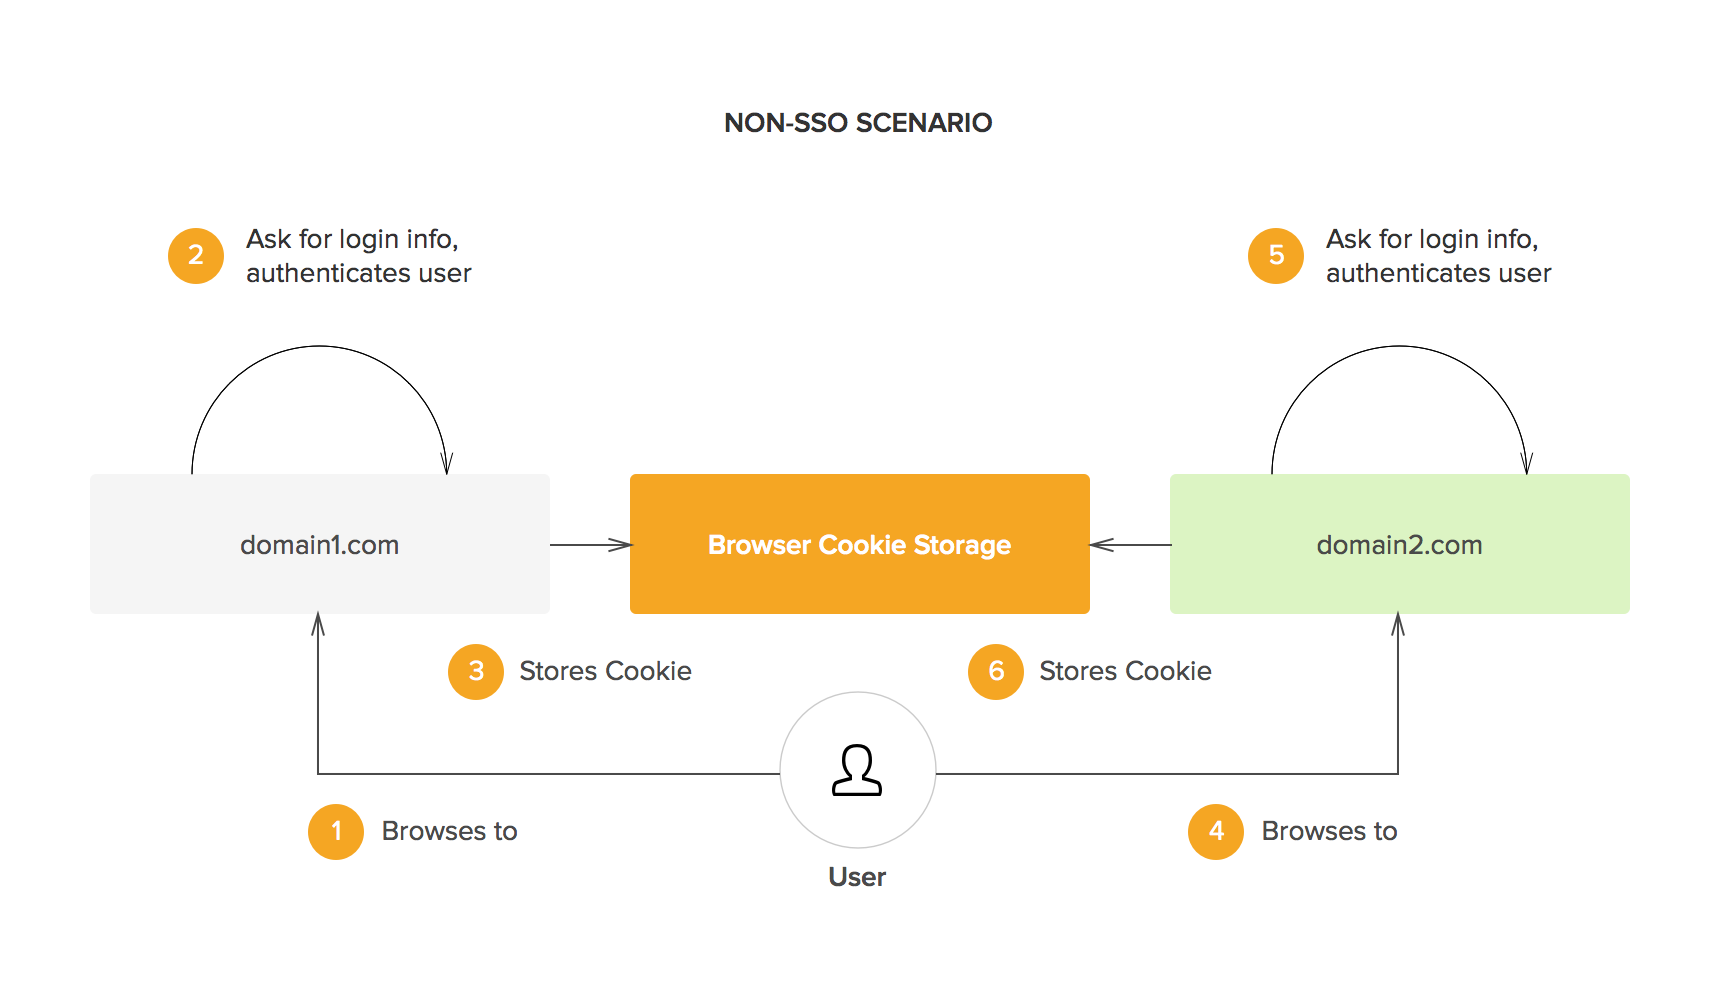
\includegraphics[width=\textwidth]{images/sso.png}
    \caption{Single Sign-on}
    \label{fig:sso}
\end{figure}

\lipsum[3]


\chapter{Implementation}
\lipsum[5]

\section{PostgreSQL}
PostgreSQL is a general purpose and object-relational database management system, the most advanced open source database system. PostgreSQL was developed based on POSTGRES 4.2 at Berkeley Computer Science Department, University of California.

PostgreSQL was designed to run on UNIX-like platforms. However, PostgreSQL was then also designed to be portable so that it could run on various platforms such as Mac OS X, Solaris, and Windows.

PostgreSQL is free and open source software. Its source code is available under PostgreSQL license, a liberal open source license. You are free to use, modify and distribute PostgreSQL in any form.

\begin{figure}
    \centering
    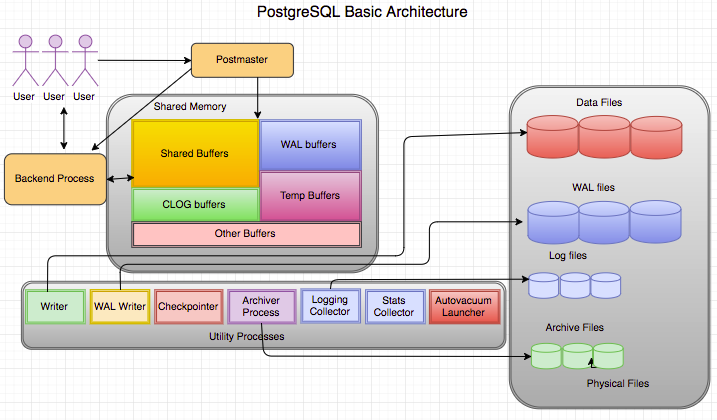
\includegraphics[width=\textwidth]{images/pg.png}
    \caption{PostgreSQL Architecture}
    \label{fig:pg}
\end{figure}

PostgreSQL requires very minimum maintenance efforts because of its stability.  Therefore, if you develop applications based on PostgreSQL, the total cost of ownership is low in comparison with other database management systems.
We utilize Postgres to store authentication and metadata information.

\lipsum[5]

\chapter{Architecture}

\blindtext[2]

\section{Gathering Data}
\lipsum[4]

\section{Data Extraction}
\subsection{Client side processing}
The crawlers does the basic work of crawling through all sets of documents where the texts are extracted  along with their absolute file location and stored in the form of a temporary dictionary. The dictionary is then sent to the search servers through REST where the indexing is done, employing a specific set of customisable analyzers and filters.

\subsection{Server side processing}
There are some of the built-in analyzers in the Elastic Search Servers, which are used to convert full-text strings into an inverted index, suitable for searching. The standard analyzer, which is the default analyzer used for full-text fields, is a good choice for most Western languages. It consists of the following:

\begin{enumerate}
    \item The standard tokenizer, which splits the input text on word boundaries
    \item The standard token filter, which is intended to tidy up the tokens emitted by the tokenizer (but currently does nothing)
    \item The lowercase token filter, which converts all tokens into lowercase
    \item The stop token filter, which removes stopwords—common words that have little impact on search relevance, such as a, the, and, is.
\end{enumerate}

The standard analyser provides for a stopword filter. It is enabled by creating a custom analyzer based on the standard analyzer and setting the stopwords parameter. We can either provide a list of stopwords or tell it to use a predefined stopwords list from a particular language.

\subsubsection{Stemmer}
Stemming attempts to remove the differences between inflected forms of a word, in order to reduce each word to its root form. For instance foxes may be reduced to the root fox, to remove the difference between singular and plural in the same way that we removed the difference between lowercase and uppercase. The root form of a word may not even be a real word. The words jumping and jumpiness may both be stemmed to jump. It doesn’t matter—as long as the same terms are produced at index time and at search time, search will just work. Elastic Search provides for default Stemmer Token filters for this purpose.

\subsubsection{Analyzer}
An analyzer examines the text of fields and generates a token stream. Analyzers are used both during ingestion, when a document is indexed, and at query time. An analyzer examines the text of fields and generates a token stream. Analyzers may be a single class or they may be composed of a series of tokenizer and filter classes. Although the analysis process is used for both indexing and querying, the same analysis process need not be used for both operations. For indexing, you often want to simplify, or normalize, words. For example, setting all letters to lowercase, eliminating punctuation and accents, mapping words to their stems, and so on. Doing so can increase recall because, for example, "ram", "Ram" and "RAM" would all match a query for "ram".

\lipsum[5]

\subsubsection{Tokenizers}
A tokenizer receives a stream of characters, breaks it up into individual tokens (usually individual words), and outputs a stream of tokens. For instance, a whitespace tokenizer breaks text into tokens whenever it sees any whitespace. It would convert the text "Quick brown fox!" into the terms [Quick, brown, fox!].
The tokenizer is also responsible for recording the order or position of each term (used for phrase and word proximity queries) and the start and end character offsets of the original word which the term represents (used for highlighting search snippets). Elasticsearch has a number of built in tokenizers which can be used to build custom analyzers.

\section{Query parsing}
We present and interface to query SQL data sources with natural language queries such as ``How many documents are present" may generate an SQL query like ``\texttt{SELECT COUNT(*) FROM document}".

This query parser is implemented as a \textit{Probabilistic Context Free Grammar}. Grammar theory to model symbol strings originated from work in computational linguistics aiming to understand the structure of natural languages. Probabilistic context free grammars (PCFGs) have been applied in probabilistic modeling of RNA structures almost 40 years after they were introduced in computational linguistics.

PCFGs extend context-free grammars similar to how hidden Markov models extend regular grammars. Each production is assigned a probability. The probability of a derivation (parse) is the product of the probabilities of the productions used in that derivation. These probabilities can be viewed as parameters of the model, and for large problems it is convenient to learn these parameters via machine learning. A probabilistic grammar's validity is constrained by context of its training dataset.

Queries are matched using weights derived from similarity score from GloVe vectors trained on Wikipedia. The knowledge engineer is expected to model the data with semantic relations. In order to handle differences in natural language queries such as the use of synonyms and inflexions, the queries are translated into GloVe vectors and a similarity score is computed using cosine vector similarity.

To model the query, we form a dependency tree from the sentences. Named entities are extracted and are used accordingly as parameters in WHERE, JOIN and GROUP BY. We perform this parsing and extraction using spaCy\cite{spacy}.

\begin{figure}
    \centering
    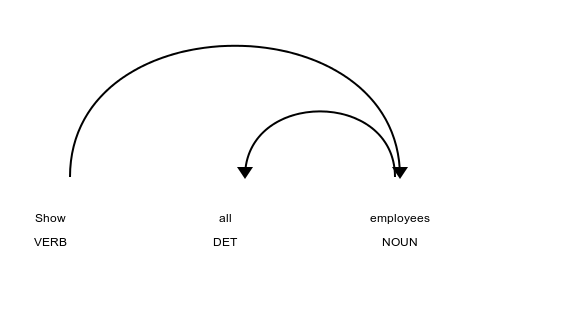
\includegraphics[width=\textwidth]{images/Show-all-employees.png}
    \caption{Parse tree for "Show all employees"}
    \label{fig:example_1}
\end{figure}

\begin{figure}
    \centering
    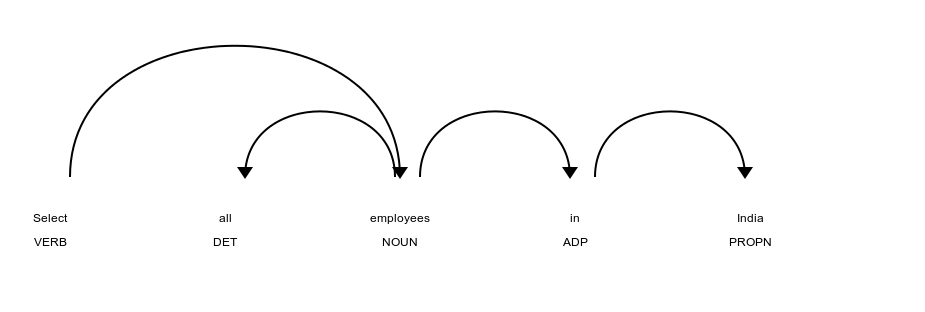
\includegraphics[width=\textwidth]{images/Select-all-employees-in-India.png}
    \caption{Parse tree for "Show all employees in India"}
    \label{fig:example_2}
\end{figure}

\begin{figure}
    \centering
    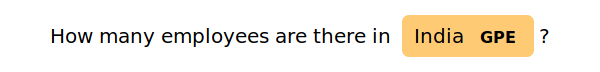
\includegraphics[width=\textwidth]{images/ent_recog.png}
    \caption{NER for "How many employees are in India"}
    \label{fig:example_2_ent}
\end{figure}

\begin{figure}
    \centering
    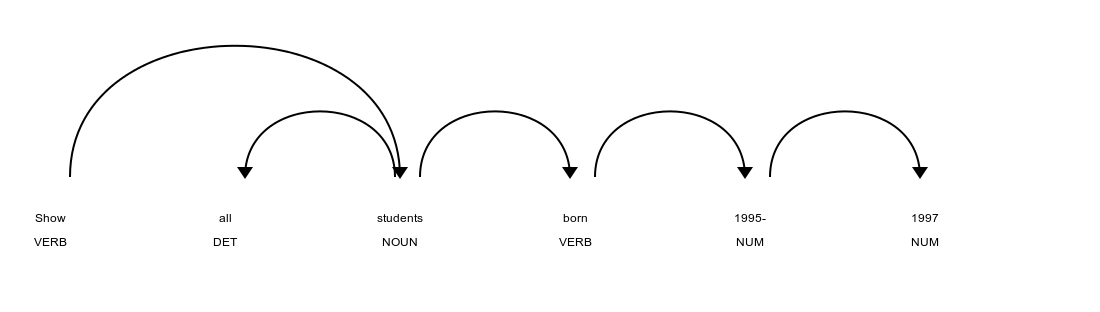
\includegraphics[width=\textwidth]{images/Show-all-students-born-1995-1997.png}
    \caption{Parse tree for "Show all students born in 1995-1997"}
    \label{fig:example_3}
\end{figure}


Some sample parse trees are shown in \autoref{fig:example_1}, \autoref{fig:example_2}, \autoref{fig:example_3} and \autoref{fig:example_2_ent}.

\section{Database results to Natural Language}

Generation of natural language\cite{popescu2003towards} from database results are made using a neural machine translation model\cite{luong2015effective}. The model is used to translate a RDF triplet into natural language. The advantage of this model is over templating methods is that this model can easily cope with unseen properties which are common in enterprise as each enterprise has its own distinct vocabulary of engineering solutions.

We model the text generation as a translation task from RDF to English. Since the sentences contain proper nouns and entities which must be preserved between translations, we preprocess the input data and delexicalize the queries and replace it with a generic marker which are replaced during relexicalization. 

\subsection{Pre-processing}

\begin{figure}
    \centering
    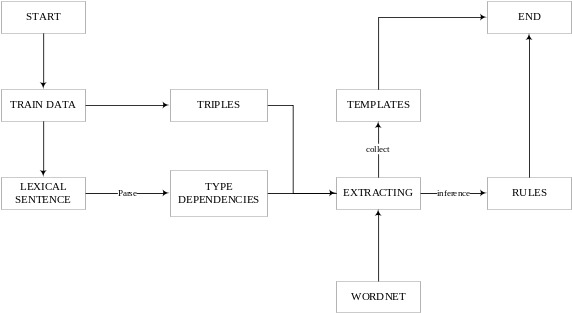
\includegraphics[width=\textwidth]{images/preprocessing.jpg}
    \caption{Entity extraction}
    \label{fig:preprocessing}
\end{figure}

\subsubsection{Determining the type of entity}

Subject and object of each triples are mapped into its type. For example: 
\begin{itemize}
    \item Donald Trump: \texttt{PERSON}
    \item 1946-06-14: \texttt{DATE}
    \item United States of America: \texttt{PLACE}
\end{itemize}

We use special treatment for detecting number and date using regular expression. For unknown entities, we use \texttt{UNKNOWN} type.

\chapter{Working}

\lipsum[5]

\section{How search works}

\lipsum[5]

\section{How database query works}
\blindtext

\chapter{Future scope}

Our solution is far from state-of-the-art and requires several improvements. 

\section{Query optimisation and improved entity extraction}
\blindtext

\section{Semantic Search}

\blindtext

\lipsum[2]

\chapter{Conclusion}
\blindtext

\bibliographystyle{unsrt}
\bibliography{references}

\end{document}
